\section{User Test}
User Tests are tests that are performed with the help of a group of people that represents a test group from the later end users. The test users have been randomly selected among students in the building. At total ten persons were asked about their opinion of the app. They have been ask to execute the following tasks before filling out about their experience with the app.
\begin{enumerate}
\item select exercise (read description and watch video)
\item learn an exercise (execute exercise ten times with coach)
\item test an exercise (stand alone exercise without help)
\item test the feedback ( is the feedback understandable? does the user's expectations on executing the exercise is reflected in the feedback )
\end{enumerate}

These tests should be executed after another. All actions combined represent a typical use case of a user.
They are only tested with one pair of smartwatch and smartphone since using the second time might influence the opinion of people and their rating of the app.

\subsection{User Test Survey}
The survey should answer the questions listed below.
\begin{itemize}
\item Is the GUI easy to understandable ?
\item is the amount of exercises, their descriptions, videos understandable ?
\item does the app assist the user appropriately ?
\item does the user have improvements/remarks
\end{itemize}

Why these questions ?\\
An app that the user does not understand is not worthy. To make sure the user knows how the app works, it is important to ask wehter the GUI is understandable.
Furthermore it is, from the health point of view, important to make sure that the user does the right movements. That is why the descriptions and videos should be understandable. Another aspect that should be tested is of well the app assists users when doing their exercise compared to exercising without the app.
Given the tester the possibility to make furher remarks for improvements makes it possible for the test user to adress aspects of the app that have not been included in the test.

\subsection{User Test Results}

%TODO results
Here are the results for user test...
\begin{figure}[b!]
  \centering
    \begin{minipage}{0.50\textwidth}
      \centering
        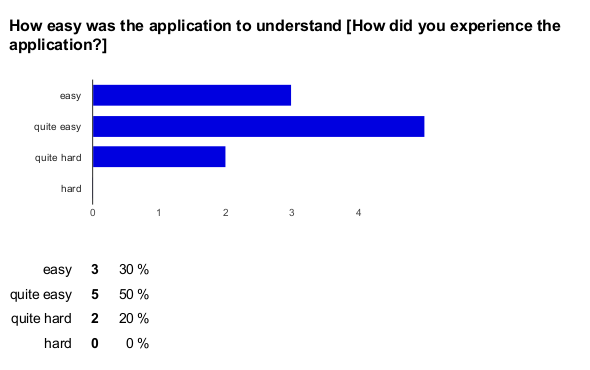
\includegraphics[width=1.80\textwidth]{00_resources/figures/survey_results1.png}
    \end{minipage}
    \begin{minipage}{0.50\textwidth}
      \centering
        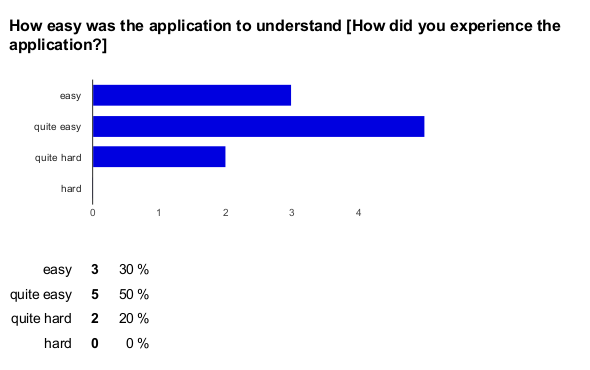
\includegraphics[width=1.80\textwidth]{00_resources/figures/survey_results1.png}
    \end{minipage}
    \begin{minipage}{0.50\textwidth}
      \centering
        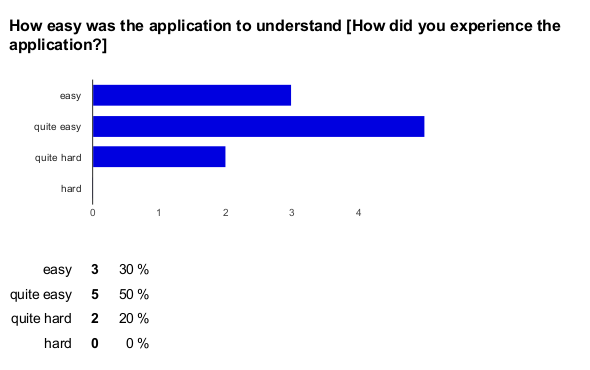
\includegraphics[width=1.80\textwidth]{00_resources/figures/survey_results1.png}
    \end{minipage}
  \caption{survey results question 3}
  \label{fig:smwui}
\end{figure}
